\section{Кластеризация слов из электронных писем}

Над содержанием электронных писем Хиллари Клинтон была также произведена кластеризация. 

Текстовый корпус, состоящий из слов из электронных писем, оказался недостаточно большим, чтобы получить хорошие результаты. Поэтому мы использовали предобученный датасет, полученный из постов в \text{Twitter} \cite{bib6}, который был дообучен словами из электронных писем.

\newpage


Результаты работы алгоритма. Ближайшие слова к <<\textit{obama}>>:

$ $

\begin{tabular}{ | l | l | }
\hline
Слово & Расстояние \\ \hline
romney & 0.9429854154586792 \\ \hline
barack & 0.9073218107223511 \\ \hline
president & 0.8986026048660278 \\ \hline
clinton & 0.8913119435310364 \\ \hline
hillary & 0.8597259521484375 \\ \hline
say & 0.8407208323478699 \\ \hline
hovv & 0.8315389752388 \\ \hline
\end{tabular}

$ $

Ближайшие слова к <<\textit{trump}>>:

$ $

\begin{tabular}{ | l | l | }
\hline
Слово & Расстояние \\ \hline
appropriator & 0.7439741492271423 \\ \hline
infighter & 0.7368026971817017 \\ \hline
zappos & 0.7316897511482239 \\ \hline
perkins & 0.7260088920593262 \\ \hline
donald & 0.7180437445640564 \\ \hline
buffett &  0.7113708853721619 \\ \hline
bloomberg & 0.7067334651947021 \\ \hline
clinton &  0.7052138447761536 \\ \hline
\end{tabular}

$ $

$  $

Так же была построена интерактивная проекция точек на \textit{2D}-плоскость с помощью алгоритма \textit{t-SNE} \cite{bib7}. \textit{t-SNE} --- это техника нелинейного снижения размерности, хорошо подходящей для вложения данных высокой размерности для визуализации в пространство низкой размерности (двух- или трехмерное). В частности, метод моделирует каждый объект высокой размерности двух- или трёхмерной точкой таким образом, что похожие объекты моделируются близко расположенными точками, а непохожие точки моделируются с большой вероятностью точками, далеко друг от друга отстоящими.

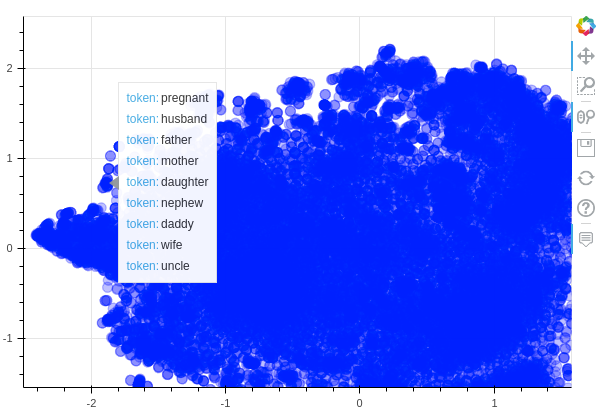
\includegraphics[scale=0.75]{pics/points.png}